When attempting to design virtual constraints for a robot, even if the goal is to generate them automatically, it is instructive and useful to have a means of examining the properties of virtual constraints and their associated partial solutions. A graphical user interface (GUI) is a particularly efficient and intuitive tool to this end. The GUI created for investigation of virtual constraints has four main features; observing the curve in Bézier space and the corresponding path in Cartesian space, investigating the shape of the partial solution given a particular virtual constraint, facilitating the slicing of the Bézier coefficient decision variable space to confirm convexity and displaying the nominal torque given a VC and an initial velocity. The GUI is also able to display the optimal coefficients based upon some start and end configuration (see Section \ref{sec:singleVCopt}) along with the graph of $\Gamma(\theta^c), \Psi(\theta^c)$ in order to investigate ordering methods (see Section \ref{sec:orderings}).

The interface is implemented in MATLAB and saves any chosen virtual constraints to the workspace. The GUI is flexible in that it is usable for any planar bipedal robot model. Figure \ref{fig:guiCG} demonstrates the typical display of the interface for the compass-gait (2-link). The software may prove useful for others to investigate the properties of virtual constraints and is therefore made freely available online, along with the other code used to generate the results for this thesis, at github.com/swardrop/virtualconstraints.

\begin{figure}
	\centering
	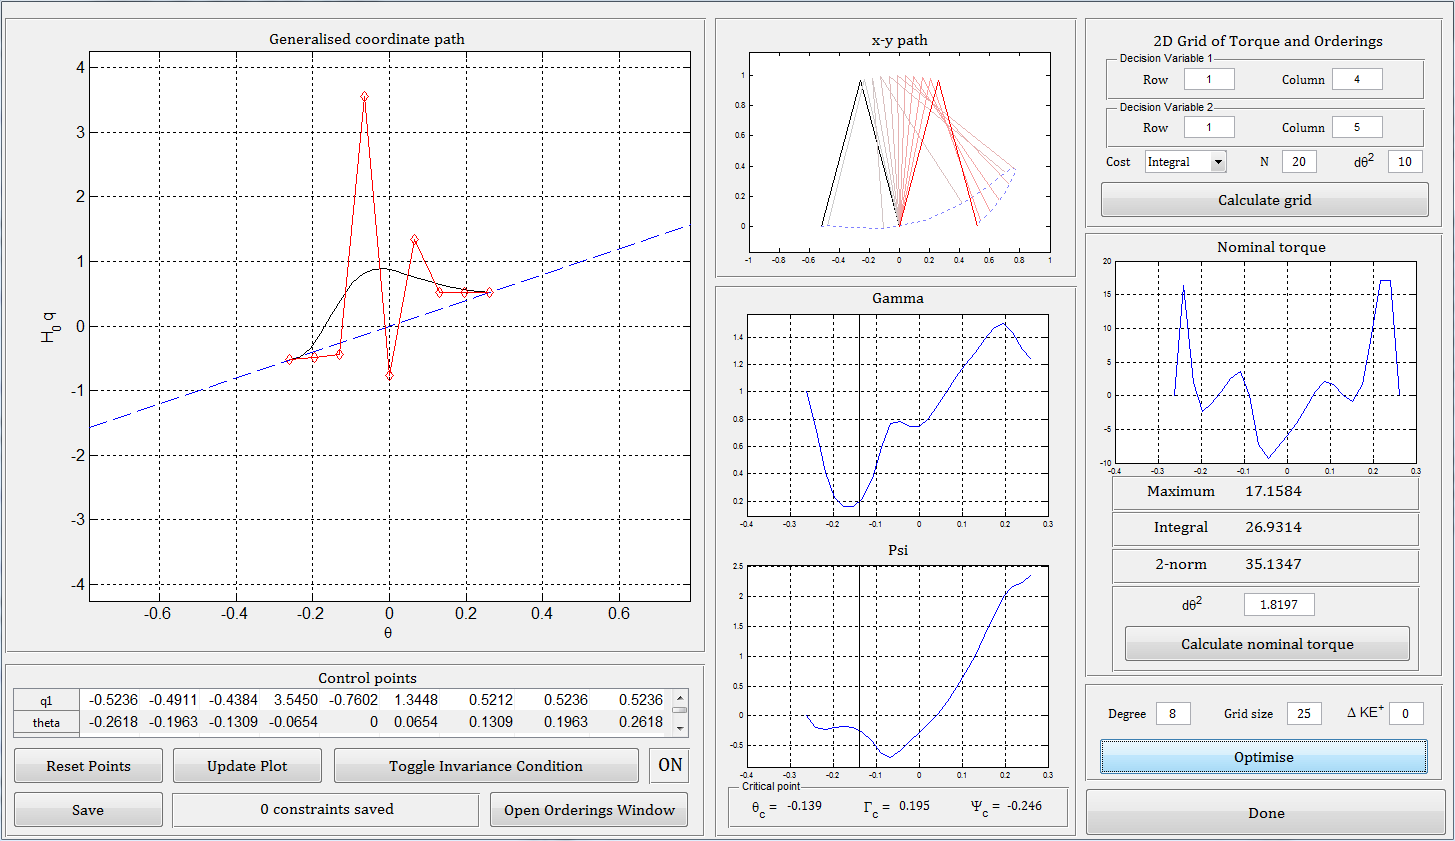
\includegraphics[width=0.9\linewidth]{4VirtConstLib/guiVC.png}
	\caption{Graphical interface for virtual constraint design showing compass-gait model}
	\label{fig:guiCG}
\end{figure}